

\documentclass[10pt,twocolumn,letterpaper]{article}

%%%%%%%%% PAPER TYPE  - PLEASE UPDATE FOR FINAL VERSION
% \usepackage{cvpr}              % To produce the CAMERA-READY version
% \usepackage[review]{cvpr}      % To produce the REVIEW version
\usepackage[pagenumbers]{cvpr} % To force page numbers, e.g. for an arXiv version
\usepackage{graphicx}     
\usepackage{subcaption}   
\usepackage{multirow}
\usepackage{tabularx}
\usepackage{booktabs}
\usepackage{colortbl}
\usepackage{amsmath}

% Import additional packages in the preamble file, before hyperref
%
% --- inline annotations
%
\newcommand{\red}[1]{{\color{red}#1}}
\newcommand{\todo}[1]{{\color{red}#1}}
\newcommand{\TODO}[1]{\textbf{\color{red}[TODO: #1]}}
% --- disable by uncommenting  
% \renewcommand{\TODO}[1]{}
% \renewcommand{\todo}[1]{#1}

\usepackage{xcolor}
\usepackage{graphicx}
\usepackage{booktabs}
\usepackage{amsmath} 
\usepackage{amsfonts}
\usepackage{amssymb}
\usepackage{multirow} 
\usepackage{makecell}
\newcommand{\shline}{\Xhline{1.1pt}} % Adjust thickness as desired

% It is strongly recommended to use hyperref, especially for the review version.
% hyperref with option pagebackref eases the reviewers' job.
% Please disable hyperref *only* if you encounter grave issues, 
% e.g. with the file validation for the camera-ready version.
%
% If you comment hyperref and then uncomment it, you should delete *.aux before re-running LaTeX.
% (Or just hit 'q' on the first LaTeX run, let it finish, and you should be clear).
\definecolor{cvprblue}{rgb}{0.21,0.49,0.74}
\usepackage[pagebackref,breaklinks,colorlinks,allcolors=cvprblue]{hyperref}


%%%%%%%%% TITLE - PLEASE UPDATE
\title{Timestep Embedding Tells: It's Time to Cache for Video Diffusion Model}

%%%%%%%%% AUTHORS - PLEASE UPDATE
\author{Feng Liu\textsuperscript{1}\thanks{Work was done during internship at Alibaba Group
.}\quad 
Shiwei Zhang\textsuperscript{2}\quad
Xiaofeng Wang\textsuperscript{1,3}\quad
Yujie Wei\textsuperscript{4}\quad
Haonan Qiu\textsuperscript{5}\\
Yuzhong Zhao\textsuperscript{1}\quad
Yingya Zhang\textsuperscript{2}\quad
Qixiang Ye\textsuperscript{1}\quad
Fang Wan\textsuperscript{1}\thanks{Corresponding author.}\\
\textsuperscript{1}University of Chinese Academy of Sciences
\quad
\textsuperscript{2}Alibaba Group\\
\textsuperscript{3}Institute of Automation, Chinese Academy of Sciences\\
\textsuperscript{4}Fudan University\quad
\textsuperscript{5}Nanyang Technological University\\
Project Page: {\color{magenta}https://liewfeng.github.io/TeaCache}}

\begin{document}
\maketitle
\begin{abstract}
Segment Anything Model 2 (SAM 2) has emerged as a powerful tool for video object segmentation and tracking anything. Key components of SAM 2 that drive the impressive video object segmentation performance include a large multistage image encoder for frame feature extraction and a memory mechanism that stores memory contexts from past frames to help current frame segmentation. The high computation complexity of multistage image encoder and memory module has limited its applications in real-world tasks, e.g., video object segmentation on mobile devices. To address this limitation, we propose EfficientTAMs, lightweight track anything models that produce high-quality results with low latency and model size. Our idea is based on revisiting the plain, nonhierarchical Vision Transformer (ViT) as an image encoder for video object segmentation, and introducing an efficient memory module, which reduces the complexity for both frame feature extraction and memory computation for current frame segmentation. We take vanilla lightweight ViTs and efficient memory module to build EfficientTAMs, and train the models on SA-1B and SA-V datasets for video object segmentation and track anything tasks. We evaluate on multiple video segmentation benchmarks including semi-supervised VOS and promptable video segmentation, and find that our proposed EfficientTAM with vanilla ViT perform comparably to SAM 2 model (HieraB+SAM 2) with $\sim$2x speedup on A100 and $\sim$2.4x  parameter reduction. On segment anything image tasks, our EfficientTAMs also perform favorably over original SAM with $\sim$20x  speedup on A100 and $\sim$20x  parameter reduction. On mobile devices such as iPhone 15 Pro Max, our EfficientTAMs can run at $\sim$10 FPS for performing video object segmentation with reasonable quality, highlighting the capability of small models for on-device video object segmentation applications. 
\end{abstract}    
\section{Introduction}
Deep learning techniques have made rapid progress in conditional image generation. For example, networks have been used to inpaint missing image regions~\citep{pathakCVPR16context,yang2016high,isola2016image}, 
add color to grayscale images~\citep{iizuka2016let,larsson2016learning,zhang2016colorful,isola2016image}, and generate photorealistic images from sketches~\cite{sangkloy2017scribbler,isola2016image}.
However, most techniques in this space have focused on generating a \textit{single} result.
In this work, we model a \textit{distribution} of potential results, as many of these problems may be multimodal in nature. For example,
as seen in Figure~\ref{fig:teaser}, an image captured at night may look very different in the day, depending on cloud patterns and lighting conditions.
We pursue two main goals: producing results which are (1) perceptually realistic and (2) diverse, all while remaining faithful to the input.

Mapping from a high-dimensional input to a high-dimensional output distribution is challenging. A common approach to representing multimodality is learning a low-dimensional latent code, which should represent aspects of the possible outputs not contained in the input image. At inference time, a deterministic generator uses the input image, along with stochastically sampled latent codes, to produce randomly sampled outputs. A common problem in existing methods is~\textit{mode collapse}~\citep{goodfellow2016nips}, where only a small number of real samples get represented in the output.
We systematically study a family of solutions to this problem.

We start with the \pp framework~\citep{isola2016image}, which has previously been shown to produce high-quality results for various image-to-image translation tasks. The method trains a generator network, conditioned on the input image, with two losses: (1) a regression loss to produce similar output to the known paired ground truth image and (2) a learned discriminator loss to encourage realism. The authors note that trivially appending a randomly drawn latent code did not produce diverse results. Instead, we propose encouraging a bijection between the output and latent space. 
We not only perform the direct task of mapping the latent code (along with the input) to the output but also jointly learn an encoder from the output back to the latent space. 
This discourages two different latent codes from generating the same output (non-injective mapping).
During training, the learned encoder attempts to pass enough information to the generator to resolve any ambiguities regarding the output mode.
For example, when generating a day image from a night image, the latent vector may encode information about the sky color, lighting effects on the ground, and cloud patterns.  Composing the encoder and generator sequentially should result in the same image being recovered. The opposite should produce the same latent code.

\begin{figure}
\centering
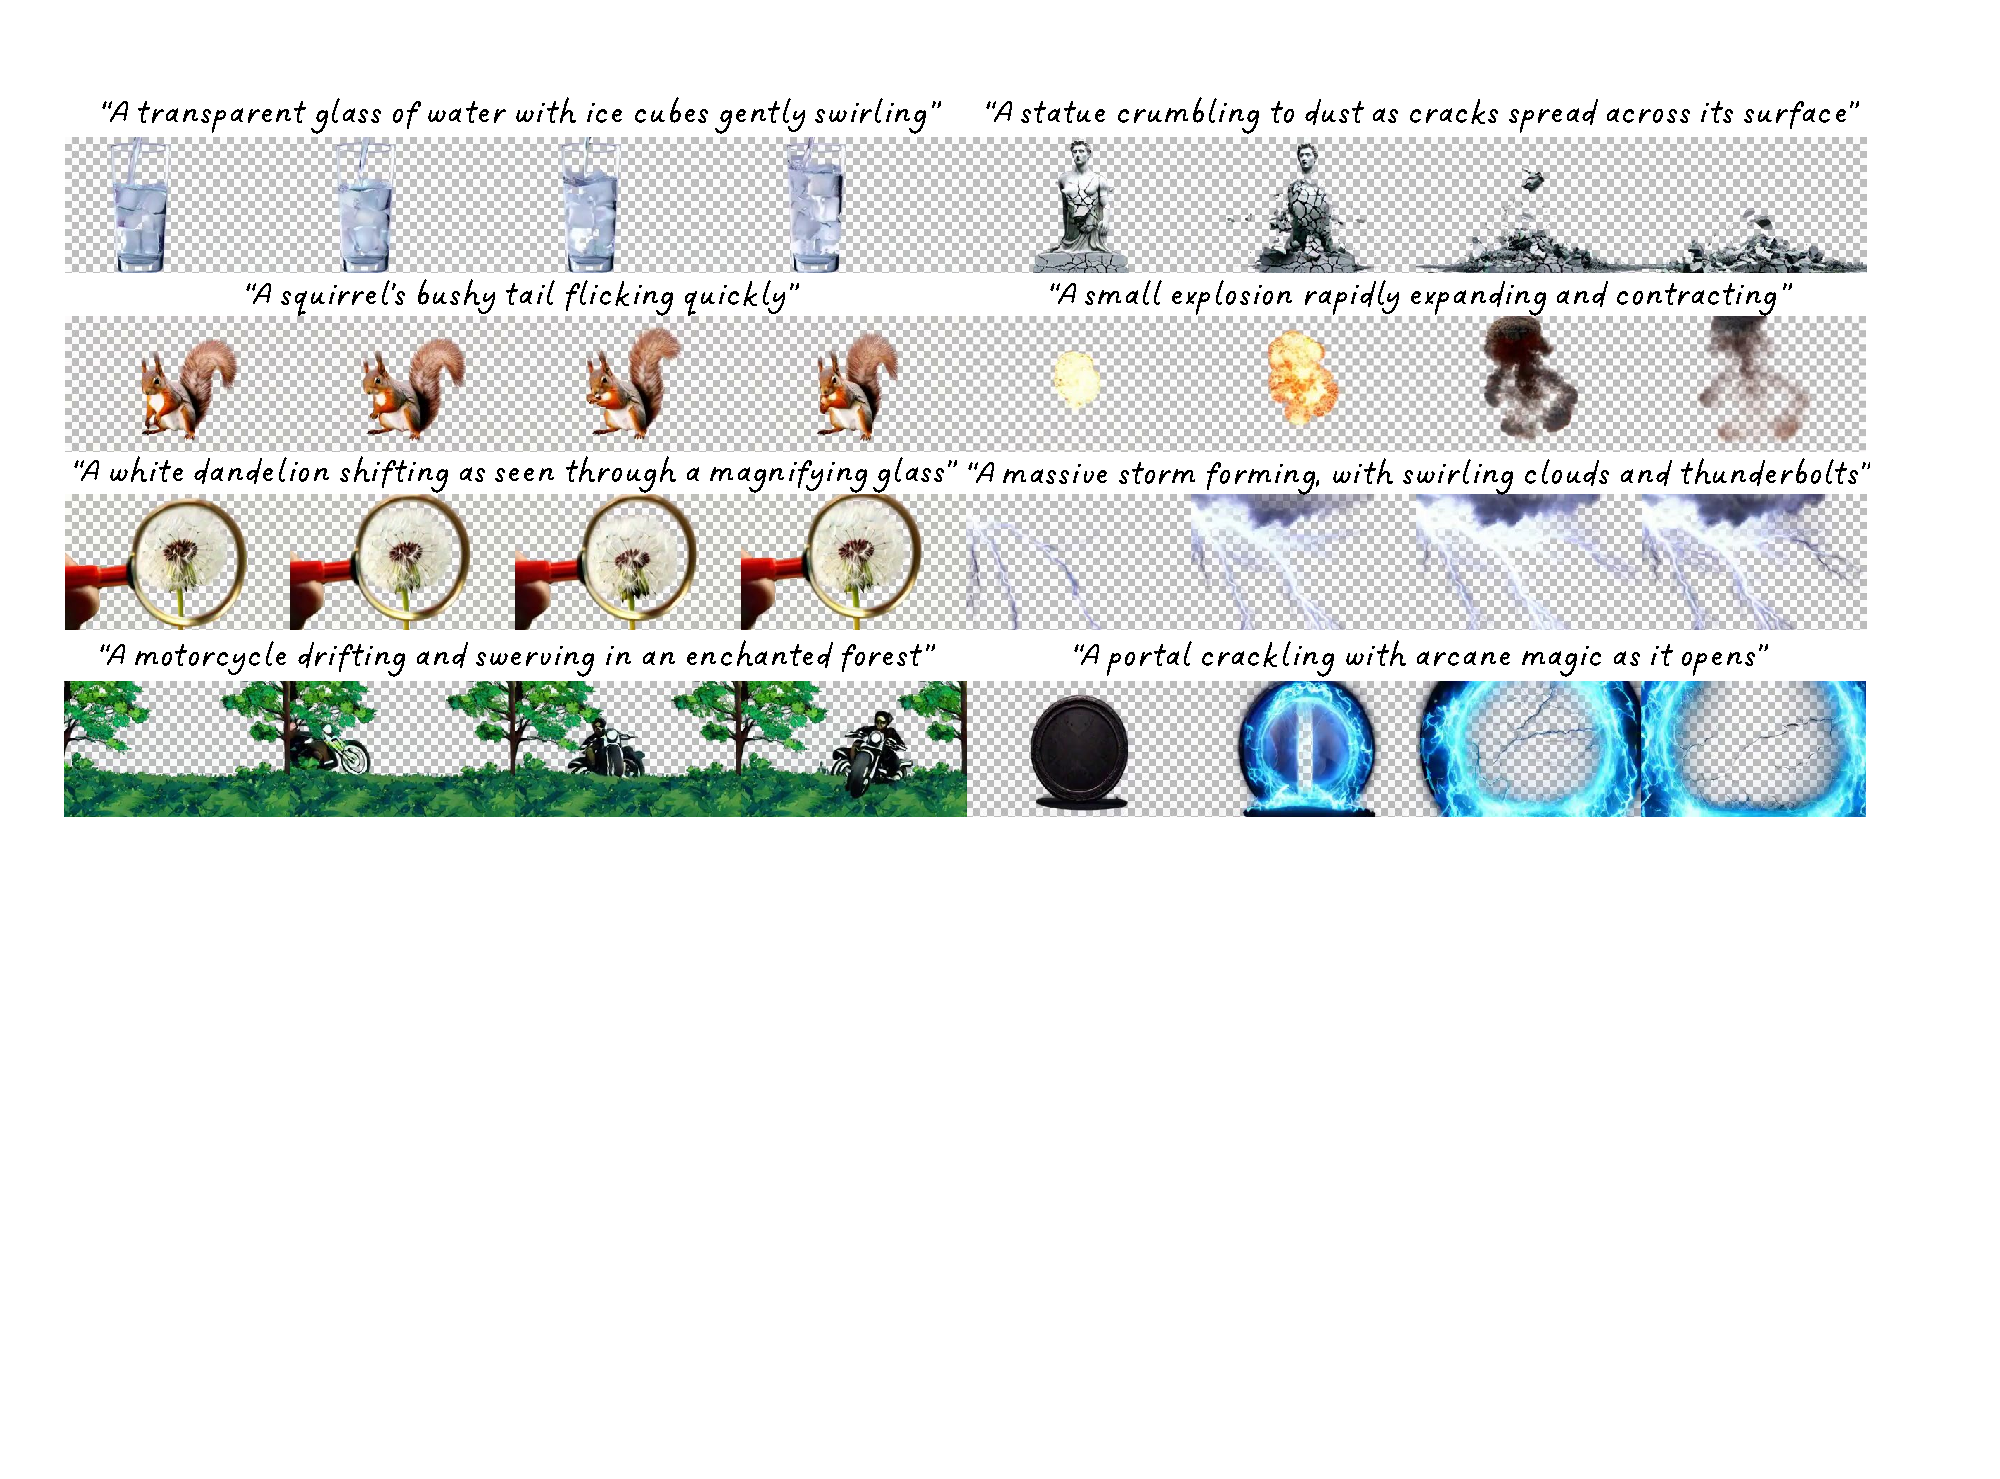
\includegraphics[width=1.\linewidth]{imgs/teaser.pdf}
\vspace{-4mm}
\caption{\small Multimodal image-to-image translation using our proposed method: given an input image from one domain (night image of a scene), we aim to model a \textit{distribution} of potential outputs in the target domain (corresponding day images), producing both realistic and diverse results.}
\vspace{-4mm}
\label{fig:teaser}
\end{figure}


In this work, we instantiate this idea by exploring several objective functions, inspired by literature in unconditional generative modeling:
  \begin{itemize}[leftmargin=0.1in]
  
    \item \textbf{\cvaegan (Conditional Variational Autoencoder GAN)}:
    One approach is first encoding the ground truth image into the latent space, giving the generator a noisy ``peek" into the desired output. Using this, along with the input image, the generator should be able to reconstruct the specific output image. To ensure that random sampling can be used during inference time, the latent distribution is regularized using KL-divergence to be close to a standard normal distribution. This approach has been popularized in the unconditional setting by VAEs~\citep{kingma2013auto} and VAE-GANs~\citep{larsen2016vaegan}.
    
    \item \textbf{\cinfogan (Conditional Latent Regressor GAN)}: Another approach is to first provide a randomly drawn latent vector to the generator. In this case, the produced output may not necessarily look like the ground truth image, but it should look realistic. An encoder then attempts to recover the latent vector from the output image. This method could be seen as a conditional formulation of the ``latent regressor" model~\citep{donahue2016adversarial,dumoulin2016adversarially} and also related to InfoGAN~\citep{xi2016infogan}.
    
    \item \textbf{\bicycle}: Finally, we combine both these approaches to enforce the connection between latent encoding and output in both directions {\em jointly} and achieve improved performance. We show that our method can produce both diverse and visually appealing results across a wide range of image-to-image translation problems, significantly more diverse than other baselines, including naively adding noise in the \pp framework. In addition to the loss function, we study the performance with respect to several encoder networks, as well as different ways of injecting the latent code into the generator network. 
\end{itemize}

We perform a systematic evaluation of these variants by using humans to judge photorealism and a perceptual distance metric~\cite{zhang2018unreasonable} to assess output diversity. Code and data are available at \url{https://github.com/junyanz/BicycleGAN}.
\section{Related Work}
\label{sec:related_work}
We briefly review prior works on fast and efficient neural networks and differentiate this work from them.

\medskip\noindent\textbf{CNN.} \enspace
CNNs are the mainstream architecture in the computer vision field, especially when it comes to deployment in practice, where being fast is as important as being accurate. Though there have been numerous studies~\cite{sifre2014rigid,singh2019hetconv,chen2019drop,chollet2017xception,zhang2017interleaved,li2021micronet,he2022tackling,zhuo2022semi} to achieve higher efficiency, the rationale behind them is more or less to perform a low-rank approximation. Specifically, the group convolution~\cite{krizhevsky2012imagenet} and the depthwise separable convolution~\cite{sifre2014rigid} (consisting of depthwise and pointwise convolutions) are probably the most popular ones. They have been widely adopted in mobile/edge-oriented networks, such as MobileNets~\cite{howard2017mobilenets,sandler2018mobilenetv2,howard2019searching},
ShuffleNets~\cite{zhang2018shufflenet,ma2018shufflenet}, GhostNet~\cite{han2020ghostnet},
EfficientNets~\cite{tan2019efficientnet,tan2021efficientnetv2}, TinyNet~\cite{han2020model}, Xception~\cite{chollet2017xception}, CondenseNet~\cite{huang2018condensenet,yang2021condensenet}, TVConv~\cite{chen2022tvconv}, MnasNet\cite{tan2019mnasnet}, and FBNet~\cite{wu2019fbnet}. While they exploit the redundancy in filters to reduce the number of parameters and FLOPs, they suffer from increased memory access when increasing the network width to compensate for the accuracy drop. By contrast, we consider the redundancy in feature maps and propose a partial convolution to reduce FLOPs and memory access \emph{simultaneously}. 

\medskip\noindent\textbf{ViT, MLP, and variants.} \enspace
 There is a growing interest in studying ViT ever since Dosovitskiy \etal~\cite{dosovitskiy2020image} expanded the application scope of transformers~\cite{vaswani2017attention} from machine translation~\cite{vaswani2017attention} or forecasting~\cite{wen2022social} to the computer vision field. Many follow-up works have attempted to improve ViT in terms of training setting~\cite{touvron2021training,touvron2022deit,steiner2021train} and model design~\cite{liu2021swin,liu2022swin,wang2021pyramid,graham2021levit,zhong2022tree}. One notable trend is to pursue a better accuracy-latency trade-off by reducing the complexity of the attention operator~\cite{ali2021xcit,vaswani2021scaling,huang2022lightvit,lu2021soft,tang2022quadtree}, incorporating convolution into ViTs~\cite{dai2021coatnet,chen2022mobile,srinivas2021bottleneck}, or doing both~\cite{cai2022efficientvit,li2022efficientformer,pan2022edgevits,mehta2022separable}. Besides, other studies~\cite{tolstikhin2021mlp,lian2021mlp,chen2021cyclemlp} propose to replace the attention with simple MLP-based operators. However, they often evolve to be CNN-like~\cite{liu2022we}. In this paper, we focus on analyzing the convolution operations, particularly DWConv, due to the following reasons: First, the advantage of attention over convolution is unclear or debatable~\cite{wang2022shift,liu2022convnet}. Second, the attention-based mechanism generally runs slower than its convolutional counterparts and thus  becomes less favorable for the current industry~\cite{mehta2021mobilevit,hu2019local}. Finally, DWConv is still a popular choice in many hybrid models, so it is worth a careful examination.
 
\section{Method}
\label{sec:method}

\begin{figure*}[t]
    \centering
    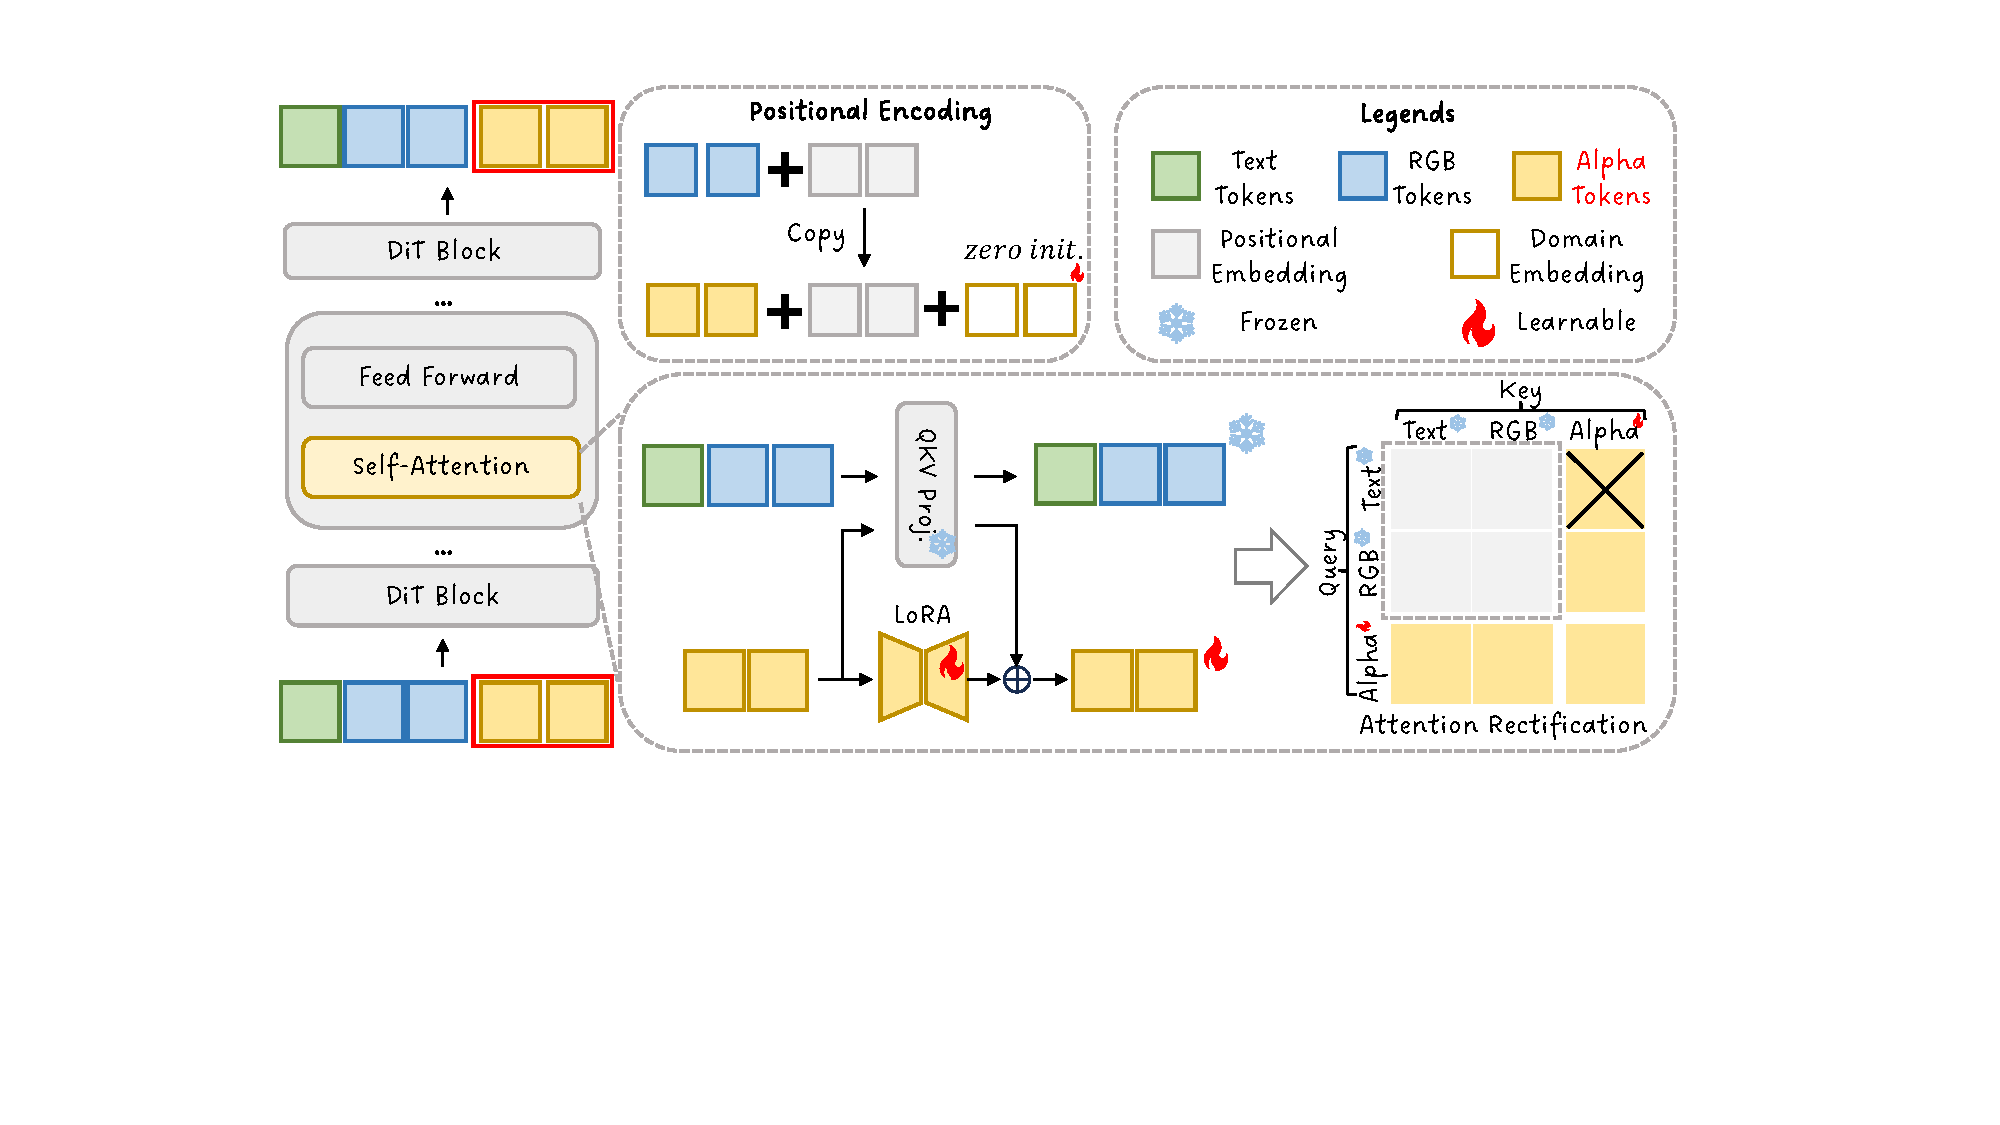
\includegraphics[width=1.0\linewidth]{figs/method-pipeline.pdf}
    \vspace{-0.2in}
    \caption{\textbf{Pipeline of TransPixar.} Our method is organized as follows: (1) \textbf{Left}: we extend the input of DiT to include new alpha tokens; (2) \textbf{Top Center}: we initialize alpha tokens with our positional encoding; (3) \textbf{Bottom Cente}r: we insert a partial LoRA and adjust attention computation during training and inference.}
    \label{fig-pipeline}
    \vspace{-0.1in}
\end{figure*}


% %-------------------------------------------------------------------------
\subsection{Preliminary}
We first introduce the open-sourced state-of-the-art DiT-based video generation models~\cite{yang2024cogvideox,genmo2024mochi}.
The core components of DiT-based video models are attention modules, and there are two primary distinctions between these models and previous approaches.
On one hand, unlike previous models that alternate between 1D temporal attention and 2D spatial attention~\cite{cerspense2023zeroscope, chen2023videocrafter1, chen2024videocrafter2, opensora}, current methods typically employ 3D spatio-temporal attention, allowing them to capture spatio-temporal dependencies more effectively.
On the other hand, instead of using cross-attention for text conditioning, these models concatenate text tokens \( \mathbf{x}_{\text{text}} \) with visual tokens \( \mathbf{x}_{\text{video}} \) into a single long sequence. 
The shape of video tokens and text tokens are \(B\times L\times D\) and \(B\times L_{\text{text}}\times D\), wher \(B\) equals to batch size, \(L_{\text{text}}\) equals to the length of text tokens, \(L\) equals to the length of video tokens and \(D\) equals to the latent dimension of transformer.
Full self-attention is then applied across the combined sequence:
\begin{equation}
\begin{aligned}
    &\text{Attention}(\mathbf{Q}, \mathbf{K}, \mathbf{V}) = \text{softmax}\left(\frac{\mathbf{Q}\mathbf{K}^T}{\sqrt{d_k}}\right)\mathbf{V}, \quad \text{where} \\
&\mathbf{Z : Z \in \{Q, K, V\}} \\&= [\mathbf{W}_{z : z \in \{q, k, v\}}(\mathbf{x}_{\text{text}}); \mathbf{f}_{z : z \in \{q, k, v\}}(\mathbf{x}_{\text{video}})]
\end{aligned}
\label{SA}
\end{equation}


Here \( \mathbf{W}_{t} \) (for \( t \in \{q, k, v\} \)) represents the projection matrixs in the transformer model, and \( \mathbf{f}_{t} \) (for \( t \in \{q, k, v\} \)) represents a combined operation that incorporates both the projection and positional encoding for visual tokens. 
There are two commonly used types of positional encoding. One is absolute positional encoding formulated as follows:
\begin{equation}
\begin{aligned}
\mathbf{f}_{z : z \in \{q, k, v\}}(\mathbf{x}_{\text{video}}) := \mathbf{W}_{z : z \in \{q, k, v\}}(\mathbf{x}_{\text{video}}^m + \mathbf{p}^m),
\end{aligned}
\label{PE}
\end{equation}
where \( \mathbf{p} \) is the positional embedding (e.g., a sinusoidal function) and \( m \) denotes the position of each RGB video token.
Another approach is the Rotary Position Embedding (RoPE)~\cite{su2024roformer}, often used by~\cite{yang2024cogvideox, genmo2024mochi}. 
This is expressed as
\begin{equation}
\begin{aligned}
\mathbf{f}_{z : z \in \{q, k\}}(\mathbf{x}_{\text{video}}) := \mathbf{W}_{z : z \in \{q, k\}}(\mathbf{x}_{\text{video}}^m) \circ e^{im\theta},
\end{aligned}
\label{RoPE}
\end{equation}
where \( m \) is the positional index, \( i \) is the imaginary unit for rotation, and \( \theta \) is the rotation angle.




% %-------------------------------------------------------------------------
\subsection{Our Approach} 
To jointly generate RGB and alpha videos, we adapt a pretrained RGB video generation model through several modifications. The whole pipeline is visualized in Fig.~\ref{fig-pipeline}.

Firstly, we double the sequence length of noisy input tokens to enable the model to generate videos of double length, from \( \mathbf{x}^{1:L}_{\text{video}} \) to \( \mathbf{x}^{1:2*L}_{\text{video}} \). 
Here, \( \mathbf{x}^{1:L}_{\text{video}} \) will be decoded into the RGB video, while \( \mathbf{x}^{L+1:2*L}_{\text{video}} \) will be decoded into the corresponding alpha video.
The Query(Q), Key(K), Value(V) representations are formulated as:
\begin{equation}
\begin{aligned}
&\mathbf{Z : Z \in \{Q, K, V\}} \\&= [\mathbf{W}_{z : z \in \{q, k, v\}}(\mathbf{x}_{\text{text}}); \mathbf{f}_{z : z \in \{q, k, v\}}(\mathbf{x}^{1:2*L}_{\text{video}})]
\end{aligned}
\end{equation}

In addition to sequence doubling, we explored increasing batch size or latent dimensions and splitting output into two domains; however, these approaches showed limited effectiveness under constrained datasets, which we discuss later.

Secondly, we modify the positional encoding function \( \mathbf{f}_{t : t \in \{q, k, v\}}(\cdot) \), as shown in Fig.~\ref{fig-pe}.
Instead of continuously numbering indices, we allow RGB and alpha tokens to share the same positional encoding. 
Taking absolute positional encoding as an example:
\begin{equation}
\begin{aligned}
&\mathbf{f}^*_{z : z \in \{q, k, v\}}(\mathbf{x}_{\text{video}}) \\:=
&\begin{cases}
\mathbf{W}_{z : z \in \{q, k, v\}}(\mathbf{x}_{\text{video}}^m + \mathbf{p}^m), & \text{if } m \leq L, \\
\mathbf{W}^*_{z : z \in \{q, k, v\}}(\mathbf{x}_{\text{video}}^m + \mathbf{p}^{m-L} + d), & \text{if } m > L.
\end{cases}
\label{eq:our_pe}
\end{aligned}
\end{equation}

Here we introduce a domain embedding \( d \), initialized to zero. We make it learnable to help the model adaptively differentiate between RGB (\(m\leq L\)) and alpha tokens (\(m>L \)). 
%
The motivation behind this design is we observe that with same postional encoding, even initializing with different noises, the tokens from two domains tend to generate same results. 
It minimizes spatial-temporal alignment challenges at the very beginning of training and thus accelerates convergence.

Next we propose a fine-tuning scheme using LoRA~\cite{hu2021lora}, in which the LoRA layer is applied only to alpha domain tokens:
\begin{equation}
\begin{aligned}
&\mathbf{W}^*_{z : z \in \{q, k, v\}}(\mathbf{x}_{\text{video}}^m + \mathbf{p}^{m-L} + d)\\=
&\ \mathbf{W}_{z : z \in \{q, k, v\}}(\mathbf{x}_{\text{video}}^m + \mathbf{p}^{m-L} + d)
\\
+\ &\gamma\cdot \text{LoRA}(\mathbf{x}_{\text{video}}^m + \mathbf{p}^{m-L} + d), \quad \text{if } m > L,
\label{eq:our_lora}
\end{aligned}
\end{equation}
where \( \gamma \) controls the residual strength. 
Additionally, we design an attention mask to block unwanted attention computation. 
Given a text-video token sequence length \( L_\text{text} + 2L \), where \( L_\text{text} \) represents text token length, the mask is defined as:
\begin{equation}
\mathbf{M}^*_{mn} = 
\begin{cases} 
-\infty, & \text{if } m \leq L_\text{text} \ \text{and} \ \, n > L_\text{text} + L, \\
0, & \text{otherwise}.
\end{cases}
\label{eq:attn_mask}
\end{equation}

Combining these modifications, inference with our method is expressed as:
\begin{equation}
\begin{aligned}
    &\text{Attention}(\mathbf{Q}, \mathbf{K}, \mathbf{V}) = \text{softmax}\left(\frac{\mathbf{Q}\mathbf{K}^T}{\sqrt{d_k}}+\mathbf{M}^*\right)\mathbf{V}, \quad \text{where} \\
&\mathbf{Z : Z \in \{Q, K, V\}} \\&= [\mathbf{W}_{z : z \in \{q, k, v\}}(\mathbf{x}_{\text{text}}); \mathbf{f}^*_{z : z \in \{q, k, v\}}(\mathbf{x}_{\text{video}})]
\end{aligned}
\label{eq:our_method}
\end{equation}

Training is carried out using flow matching~\cite{liu2022flow} or a traditional diffusion process~\cite{ho2020denoising}.


\begin{figure}[t]
    \centering
    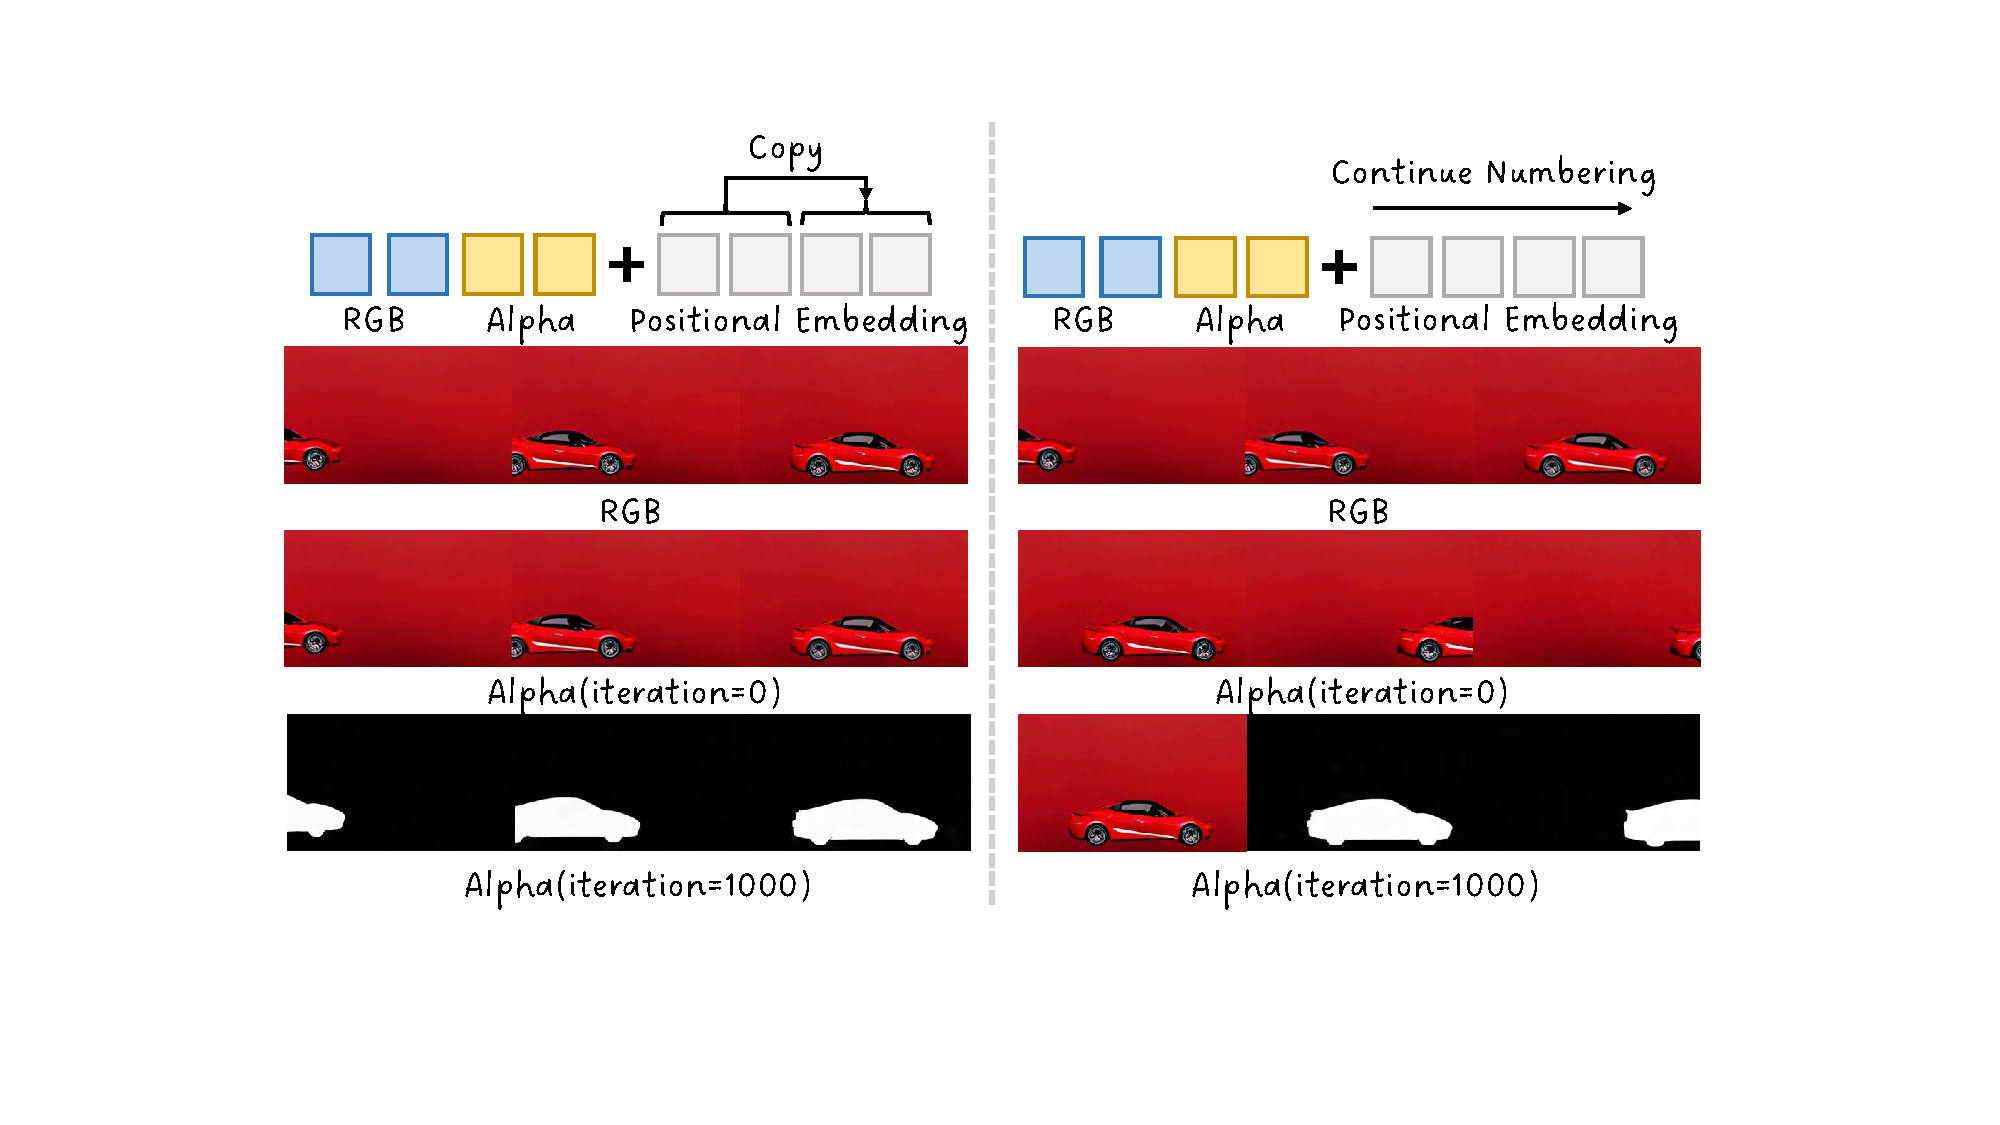
\includegraphics[width=1.0\linewidth]{figs/method-pe_init.pdf}
    \vspace{-0.2in}
    \caption{\textbf{Positional Encoding Design for RGBA Generation.} Assigning alpha tokens the same positional encoding as RGB yields similar results, resulting in faster convergence after 1000 iterations compared to standard encoding strategies.}
    \label{fig-pe}
    \vspace{-0.1in}
\end{figure}

% %-------------------------------------------------------------------------
\subsection{Analysis}
% % given our goal is 最大程度地继承 pretrain video model的能力,让它能生成的东西超越已有的RGBA训练集,
% 在目前我们使用的3d full attention DiT的video generation model的框架下,最重要的计算是attention mechanism,因此我们进一步对该过程进行分析:
% The attention matrix, \(\mathbf{Q}\mathbf{K}^T\), now has dimensions \((L_\text{text} + 2*L) \times (L_\text{text} + 2*L)\), which we simplify by organizing it into a 3x3 grouped attention matrix—\textbf{Text-attend-to-RGB}, \textbf{RGB-attend-to-Text}, and so forth, as illustrated in Fig.~\ref{fig-pipeline}. Then we procceed to analyze them:

% \noindent{\textbf{Text-Attend-to-RGB} and \textbf{RGB-Attend-to-Text}}.
% Given this matrix, we are supposed to preserve as much of the computation in the upper-left 2x2 section as possible so that we can preserve the RGB generation potential. 

% These represent the upper-left 2x2 section in \(\mathbf{Q}\mathbf{K}^T\) and 是RGB original generation model有且仅有的计算过程,如果我们能保证这部分计算不受影响,we can replicate the original RGB generation performance. 
% Therefore, we limited the scope of LoRA's influence, as defined in Equation~\eqref{eq:our_lora}, we retain the original QKV values for both text and RGB tokens, maintaining the pretrained model’s behavior in these domains.

% Besides the partial lora, the introduction of alpha tokens make the text and RGB tokens need to act as key and interact with alpha tokens as query, which will also 改变这个2x2 attention matrix的计算结果。
% Therefore, we proceed to analyze two additional attention computations that affect RGB generation shown in Fig.~\ref{fig-attn}:


% \noindent{\textbf{Text-Attend-to-Alpha}}: We find this attention is detrimental to the generation quality. 
% Since the model is originally trained with text and RGB data, introducing attention from text to alpha causes interference due to the domain gap between alpha and RGB. 
% Specifically, alpha modality provide only contour information and lack the rich texture, color, and semantic details associated with text prompt, thereby degrading generation quality. 
% To mitigate this, we design the attention mask (Equation~\eqref{eq:attn_mask}) that blocks this computation.

% \noindent{\textbf{RGB-Attend-to-Alpha}}: In contrast, we identify \textbf{RGB-to-Alpha} as essential for successful joint generation. 
% This attention allows the model to refine RGB tokens by considering alpha information, facilitating alignment between generated RGB and alpha channels. 
% This refinement process is a critical component missing in prior generation-then-prediction pipelines, which lack a feedback mechanism for RGB refinement based on alpha guidance.
Given our goal of maximizing the inherited capabilities of the pretrained video model, enabling it to generate beyond the existing RGBA training set, we analyze the most critical component within our current 3D full attention DiT video generation model: the attention mechanism.
%
The attention matrix, \(\mathbf{Q}\mathbf{K}^T\), has dimensions \((L_\text{text} + 2*L) \times (L_\text{text} + 2*L)\), which we simplify by organizing it into a 3x3 grouped attention matrix—including \textbf{Text-attend-to-RGB}, \textbf{RGB-attend-to-Text}, and so forth, as illustrated in Fig.~\ref{fig-pipeline}. %We then analyze these components:

\vspace{0.5em}
\noindent\textbf{Text-Attend-to-RGB and RGB-Attend-to-Text}. These represent the upper-left 2x2 section of  and are computations that exist solely in the original RGB generation model. If we ensure that this part of the computation remains unaffected, we can replicate the original RGB generation performance. Therefore, we limit the scope of LoRA's influence, as defined in Eq.~\eqref{eq:attn_mask}, by retaining the original QKV values for both text and RGB tokens, thus preserving the pretrained model’s behavior in these domains.

Besides the partial LoRA, the added alpha tokens requires the text and RGB tokens to also act as queries and interact with the alpha tokens as keys, which alters the computation in this 2x2 attention matrix. 
Therefore, we further analyze two additional attention computations that impact RGB generation, as shown in Fig.~\ref{fig-attn}.

\vspace{0.5em}
\noindent\textbf{Text-Attend-to-Alpha.} We find that this attention is detrimental to the generation quality. Since the model was originally trained with text and RGB data, introducing attention from text to alpha causes interference due to the domain gap between alpha and RGB. Specifically, the alpha modality provides only contour information and lacks the rich texture, color, and semantic details associated with the text prompt, thereby degrading generation quality. To mitigate this, we design the attention mask (Eq.~\eqref{eq:attn_mask}) that blocks this computation.

\vspace{0.5em}
\noindent\textbf{RGB-Attend-to-Alpha.} In contrast, we identify \textbf{RGB-to-Alpha} as essential for successful joint generation. This attention allows the model to refine RGB tokens by considering alpha information, facilitating alignment between generated RGB and alpha channels. This refinement process is a critical component missing in previous generation-then-prediction pipelines, which lacked a feedback mechanism for RGB refinement based on alpha guidance.


\begin{figure}[t]
    \centering
    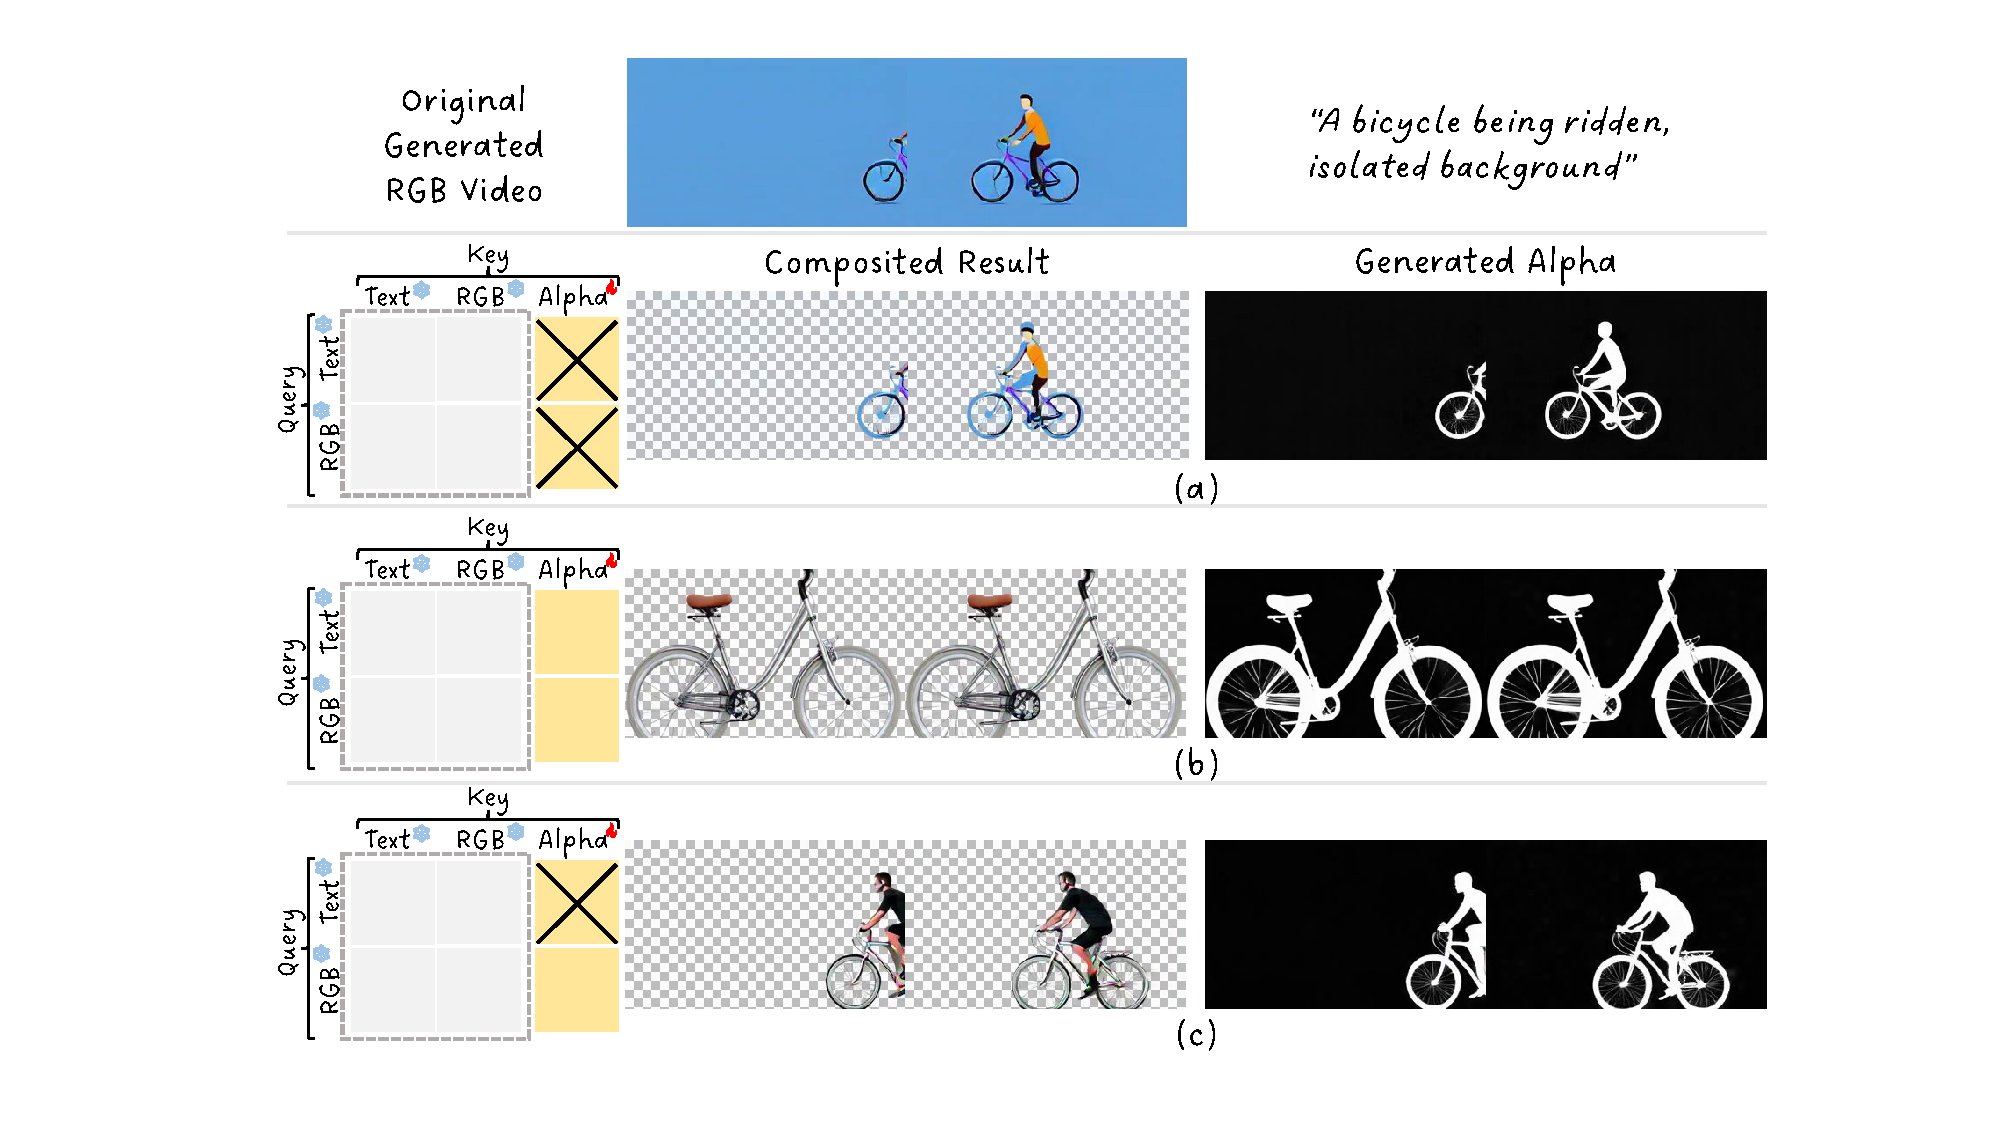
\includegraphics[width=1.0\linewidth]{figs/method-attn.pdf}
    \vspace{-0.2in}
    \caption{\textbf{Attention Rectification.} (a) Eliminating all attention from alpha as a key preserves 100\% RGB generation but leads to poor alignment. (b) Retaining all attention significantly degrades quality, causing a lack of motion in bicycles. (c) Our method achieves an effective balance.
    }
    \label{fig-attn}
    \vspace{-0.1in}
\end{figure}




%
% --- inline annotations
%
\newcommand{\red}[1]{{\color{red}#1}}
\newcommand{\todo}[1]{{\color{red}#1}}
\newcommand{\TODO}[1]{\textbf{\color{red}[TODO: #1]}}
% --- disable by uncommenting  
% \renewcommand{\TODO}[1]{}
% \renewcommand{\todo}[1]{#1}

\usepackage{xcolor}
\usepackage{graphicx}
\usepackage{booktabs}
\usepackage{amsmath} 
\usepackage{amsfonts}
\usepackage{amssymb}
\usepackage{multirow} 
\usepackage{makecell}
\newcommand{\shline}{\Xhline{1.1pt}} % Adjust thickness as desired

\section{Experiments}
\label{sec:experiments}

We present results for supervised video classification and self-supervised masked auto-encoding with frozen representations evaluated on two downstream tasks: video classification and point tracking. To analyse the memory capabilities of our model, we also include a reconstruction task of frames seen in the distant past. Using the same task, we study the generalisation capabilities to longer sequences than seen during training. We follow the ViT scaling configurations and, unless otherwise stated, we use the \textbf{B}ase version for our model for all our experiments. We specify the number of parameters for all models considered in our experiments, and we include in the supplementary material all the training hyperparameters and data augmentations used in all experiments.

\subsection{Supervised video classification}

\par \noindent \textbf{Datasets:}
We use large-scale real-world datasets for the supervised video classification task. Kinetics400~\citep{Carreira_2017_CVPR} contains 241,512 videos\footnote{Kinetics is a dynamic dataset (videos may be removed from
YouTube). Our current version has 241,512 videos, compared to 267,000 videos reported in~\cite{vivit}, so a decrease of almost 10\%, noticeable in the final performance.} across train, validation, and test splits, 10s-long (25fps), spanning 400 classes. This dataset is known to require modelling appearance for successful action recognition. To challenge our model's capability of understanding motion, we also use SSv2 dataset~\citep{goyal2017something}, which contains 220,847 shorter videos (2-6s long), sampled at 12fps, representing 174 classes. This dataset includes actions that differ in finer motion-related details, requiring a deeper temporal understanding, e.g. \textit{pouring something into something} vs \textit{pretending to pour something into something}. 

\par \noindent \textbf{Baselines:}
We use ViViT~\citep{vivit} as our main baseline. We consider the full self-attention version, which patchifies and flattens the entire video, prepends a video class token, then runs self-attention blocks. We also consider the factorised encoder version (ViViT FE), which runs a ViT image model over all the frames, and uses temporal self-attention blocks to integrate the information over time. Finally, we also consider a baseline that uses only LRU recurrent and MLP blocks, configured similar to VideoMamba~\cite{li2024videomambastatespacemodel}, i.e. it does not use self-attention blocks, denoted \textit{PureLRU}. Similar to ViViT, this model first patchifies and flattens the video, prepends a class token, then applies a sequence of recurrent blocks. All baselines use learnt spatio-temporal positional encoding, whereas the proposed \ssm\ uses only spatial positional encoding as the temporal dimension is implicitly modelled through its recurrence.


\par \noindent \textbf{Results:} We include results for training from scratch or using Imagenet pre-trained weights to initialise the weights of the ViT blocks. Figure~\ref{fig:baselines} shows a first comparison between \ssm\ and the above baselines, with all models being trained from scratch on supervised classification on SSv2. We consider the \textbf{S}mall version for all models as the larger \textbf{B}ase version shows stability issues when trained from scratch, as reported in other works as well~\cite{li2024videomambastatespacemodel,vivit}. As expected, the performance on this challenging dataset when training from scratch is far from SOTA, but it clearly shows that the proposed factorisation has superior video modelling capabilities compared to baselines, ViViT-S with full self-attention being the closest competitor. PureLRU's performance is very poor, which is in line with the findings of other works (\eg VideoMamba) who report that bidirectional (non-causal) processing of the input is needed for good performance. 

We report further results comparing against ViViT-B and ViViT-L with full self-attention when using Imagenet pre-trained weights; see Table~\ref{tab:ssv2} for SSv2 results and Table~\ref{tab:kinetics} for Kinetics400 results.
We can observe that our model achieves better performance compared to ViViT baselines on SSv2, but it is slightly below ViViT-L on Kinetics400. This result could reflect the difference between the two datasets mentioned above: outperforming ViViT-L on SSv2 suggests that \ssm\ is superior at modelling motion compared to ViViT, but on Kinetics where the appearance is enough for successful classification, both models are on par. We consider this to be a strong positive result for our model given that it has about 3x less parameters compared to ViViT-L and significantly lower FLOPs count and memory footprint as shown in Figure~\ref{fig:memory}.

\begin{figure}[t]
  \centering
  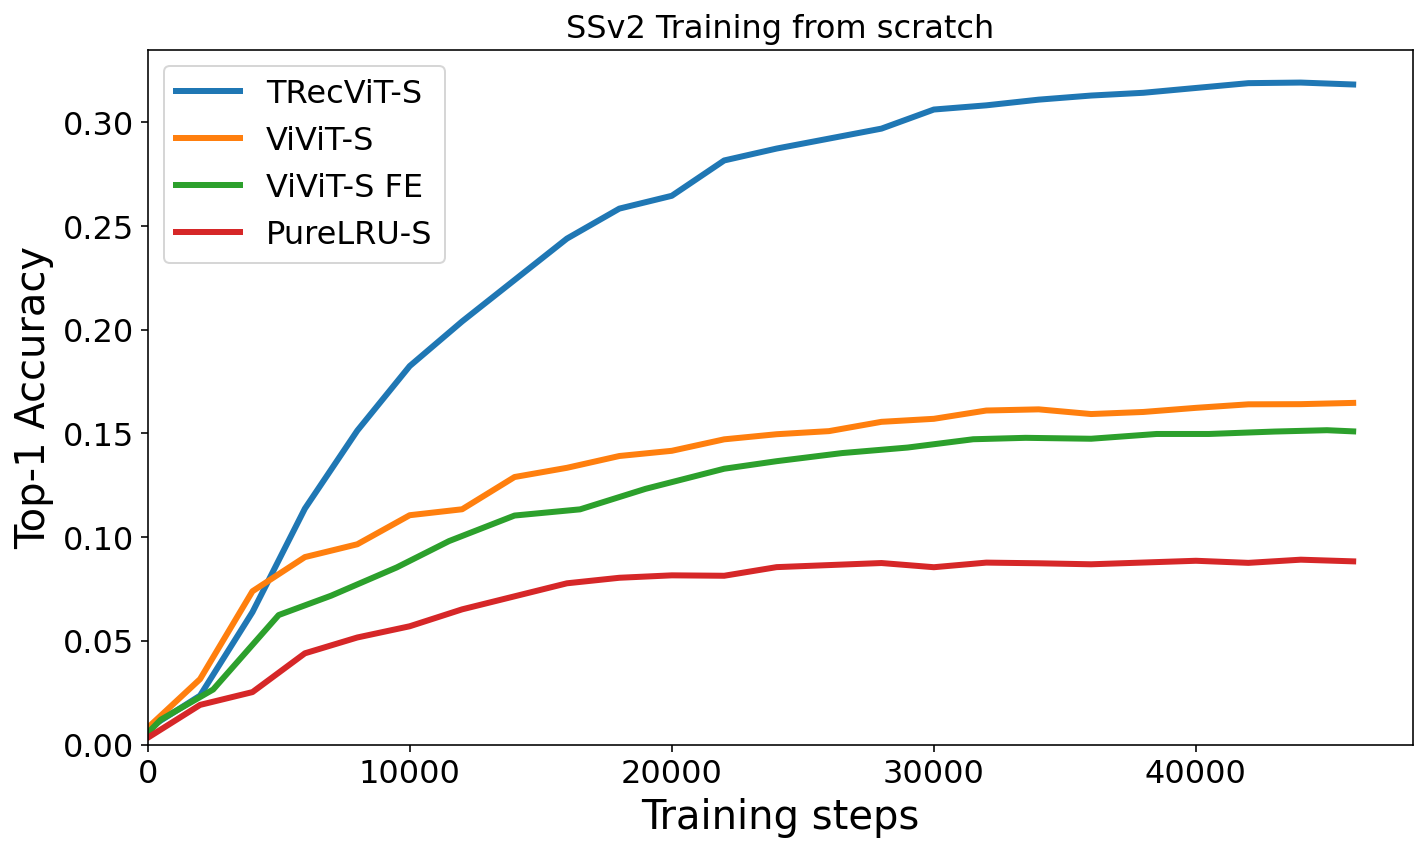
\includegraphics[width=.9\linewidth]{img/scratch.png}
  \caption{\ssm\ compared to baselines on supervised video classification on SSv2 dataset, trained from scratch. The plot shows the evolution of the evaluation accuracy as training progresses.
  }

  \label{fig:baselines}
\end{figure}
 

 \begin{figure*}[h]
  \centering
  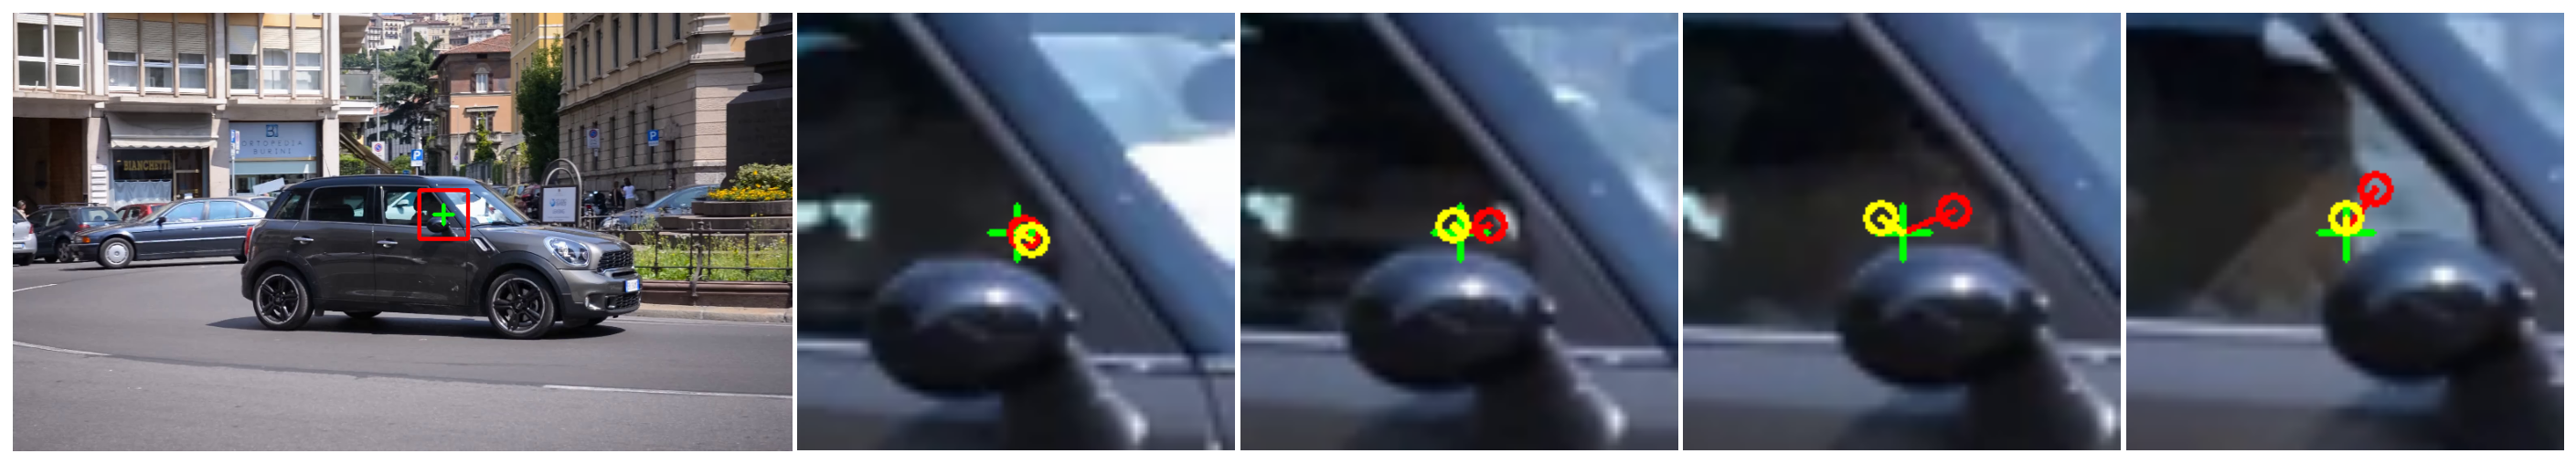
\includegraphics[width=\linewidth]{img/davis.png}
  \caption{Qualitative results obtained by \ssm\ for point tracking on DAVIS dataset compared to VideoMAE. The leftmost image indicates the point to track in the original frame, and the images towards the right show zoom-ins on subsequent frames. Green plus (+) marker indicates the ground truth, yellow circle indicates \ssm's predictions and red circles indicate VideoMAE's predictions.}
  \label{fig:tracking}
\end{figure*}


\begin{table}
    \centering
    \small{
    \begin{tabular}{l|c|c|r}
    \hline
    \textbf{Model} & \textbf{Patch size} & \textbf{Top-1 acc (\%)} & \textbf{\# params} \\
    \hline
    ViViT-B & (2, 16, 16) & 59.1 & 90M \\
    ViViT-L & (2, 16, 16) & 65.9 & 320M \\
    \ssm\ & (1, 16, 16) & \textbf{66.8} & 109M\\
    \hline
    \end{tabular}}
    \caption{Performance of \ssm\ compared to ViViT-B and ViViT-L baselines on SSv2 dataset with all models initialised from Imagenet pre-training. For ViViT-L, we use the result reported by its authors, for ViViT-B we obtained the results internally as they were not reported in the original paper for this dataset.}
    \label{tab:ssv2}
    \end{table}
    
\begin{table}
    \centering
    \small{
    \begin{tabular}{l|c|c|r}
    \hline
    \textbf{Model} & \textbf{Patch size} & \textbf{Top-1 acc (\%)} & \textbf{\# params} \\
    \hline
    ViViT-B & (2, 16, 16) & 78.1 & 90M \\
    ViViT-L & (2, 16, 16) & \textbf{78.7} & 320M \\
    \ssm\ & (1, 16, 16) & 78.4 & 109M\\
    \hline
    \end{tabular}}
    \caption{Performance of \ssm\ compared to ViViT-B and ViViT-L baselines on Kinetics400 dataset, with all models initialised from Imagenet pre-training. For ViViT-B and ViViT-L, we include the result we obtained internally by re-training the model on the current Kinetics400 dataset version; see footnote. In the original paper, the authors reported 80.3\% on Kinetics400 for ViViT-L.}
    \label{tab:kinetics}
    \end{table}

\subsection{Self-supervised masked autoencoding}
\label{sec:mae}
We use Kinetics400 for self-supervised pre-training from scratch and we report results on multiple downstream datasets and tasks by fine-tuning attention readout heads on top of frozen representations. We choose this setup, as opposed to fine-tuning end-to-end, as the  performance in this case more clearly reflects the quality of the pre-trained representations. As mentioned in the previous section, we use a large masking ratio (0.90), which makes pre-training very efficient. We report the number of parameters for every model considered. Note that the number of parameters for \ssm\ is different from the one reported in the previous section due to the addition of the readout heads.

\par \noindent \textbf{Video classification:}  We report video classification accuracy as downstream task using attention readout heads on SSv2 and Kinetics400. We compare the performance against VideoMAE-L~\cite{tong2022videomae} in Table~\ref{tab:selfsup}. Our model obtains slightly better performance on both datasets compared to this strong baseline, despite having almost 3$\times$ less parameters. 

\par \noindent \textbf{Point tracking:} To demonstrate that our model can handle dense(r) tasks as well, we evaluate the same frozen MAE representations for the point tracking task. We use the recurrent architecture in MooG~\cite{steenkiste2024moving} as a readout due to its simplicity. MooG uses light cross-attention layers to process the embeddings of each frame in order, and the readout state is carried over through time. We finetune the MooG readout head using MOVi-E dataset~\cite{movie} as done in popular point tracking works~\cite{DoerschYVG0ACZ23}. We evaluate these fine-tuned representations on two datasets: Perception Test~\citep{patraucean2023perception} and DAVIS dataset~\cite{davis2017} with point tracks extracted in~\cite{doersch2022tapvid}. We report average Jaccard metric~\cite{doersch2022tapvid} for \ssm\ compared with MooG and VideoMAE; see Table~\ref{tab:pt}. \ssm\ obtains better performance on both datasets compared to baselines, which reinforces the observation that our proposed model has strong motion modelling capabilities. We include qualitative results for this task in Figure~\ref{fig:tracking}. We can observe that the results are visibly better compared to VideoMAE. More visualisations are included in the supplementary material.

\begin{table}
    \centering
    \small{
    \begin{tabular}{l|c|c|r}
    \hline
    \textbf{Model} & \textbf{Dataset} & \textbf{Top-1 acc (\%)} & \textbf{\# params} \\
    \hline
    VideoMAE & Kinetics400 & 45.8 & 330M \\
    \ssm\ & Kinetics400 & \textbf{46.0} & 128M\\
    \hline
    \hline
    VideoMAE & SSv2 &  53.7 & 330M \\
    \ssm\ & SSv2 &  \textbf{53.9} & 128M\\
    \hline
    \end{tabular}}
    \caption{Performance of \ssm\ compared to VideoMAE on video classification using frozen MAE representations, pre-trained on Kinetics400.}
    \label{tab:selfsup}
    \end{table}

\begin{table}
    \centering
    \small{
    \begin{tabular}{l|c|c|c|r}
    \hline
    \textbf{Model} & \textbf{Dataset} & \textbf{\# frames} & \textbf{AJ} & \textbf{\# params} \\
    \hline
    MooG & DAVIS & 8 & 0.687 & 35M \\
    VideoMAE & DAVIS & 8 & 0.703 & 330M \\
    \ssm\ & DAVIS & 8 & \textbf{0.706} & 128M\\
    
    \hline
    \hline
    MooG & Perception Test & 16 & 0.760 & 46.5M \\
    VideoMAE & Perception Test & 16 & 0.761 & 330M \\
    \ssm\ & Perception Test & 16 & \textbf{0.783} & 128M\\
    \hline
    \end{tabular}}
    \caption{Performance of \ssm\ compared to baselines on point tracking task on DAVIS and Perception Test datasets. All models use frozen representations evaluated using the readout head from MooG.}
    \label{tab:pt}
    \end{table}

\begin{figure*}[h]
  \centering
  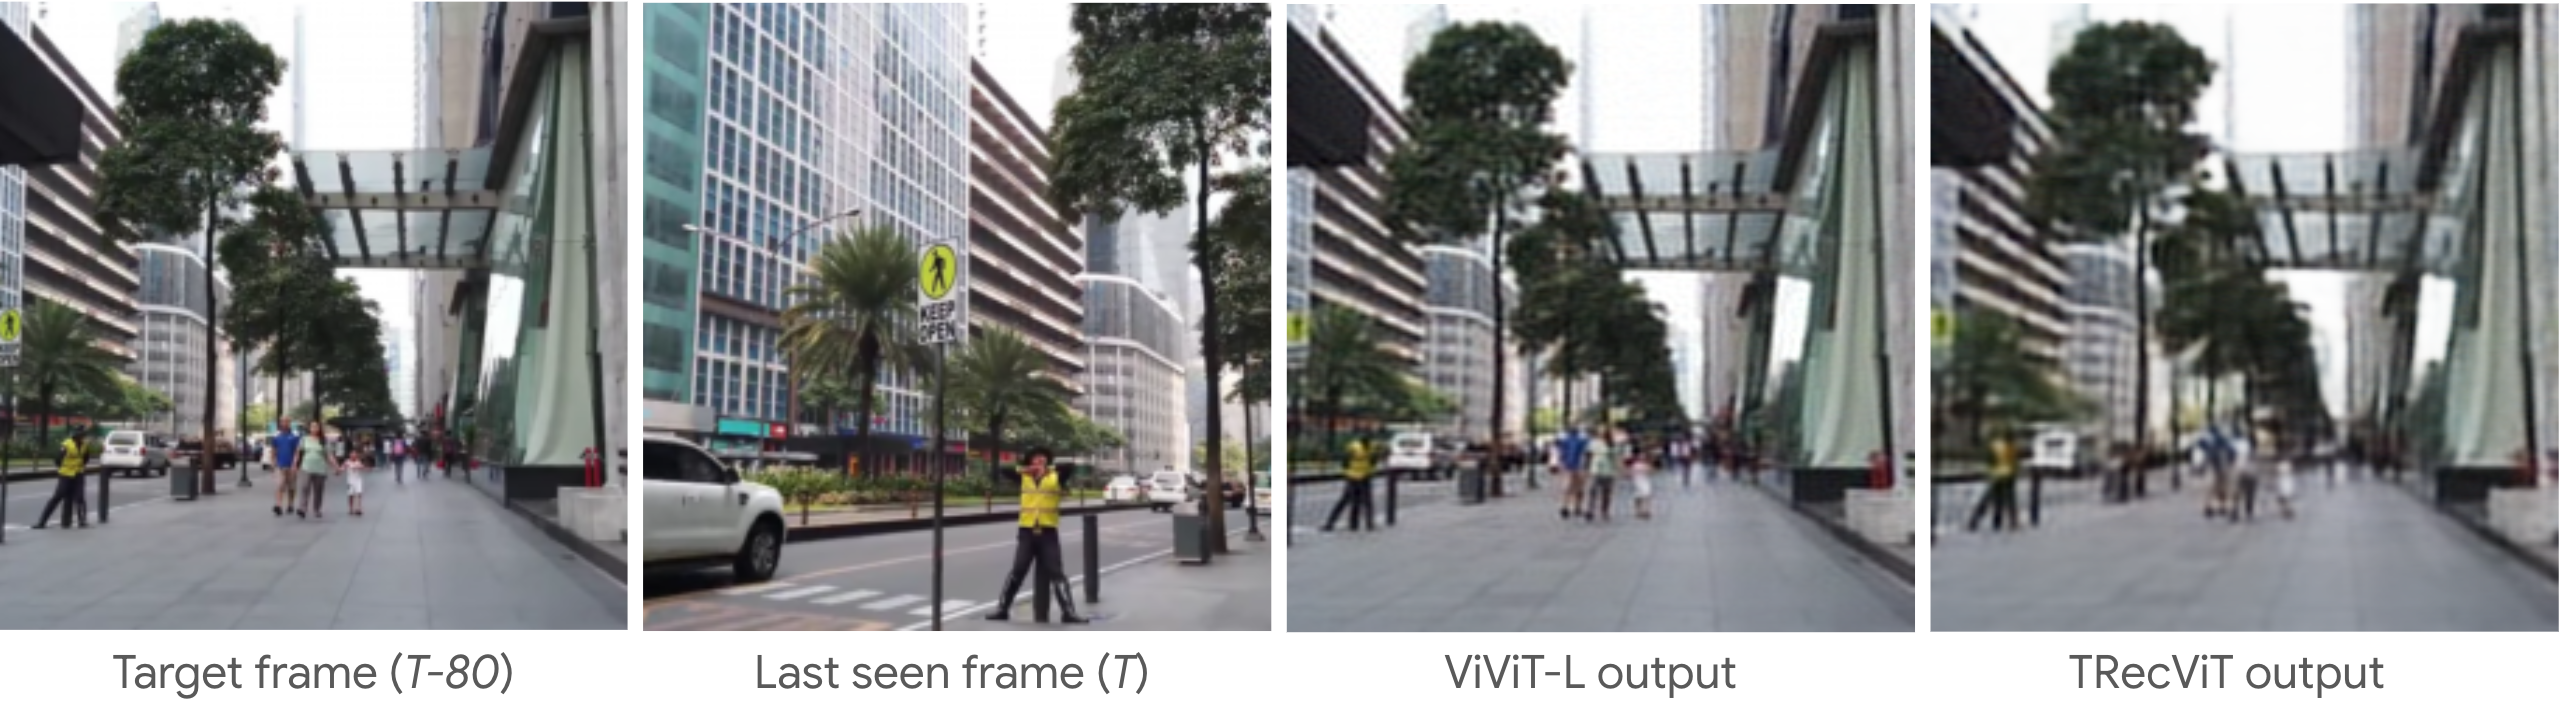
\includegraphics[width=\linewidth]{img/wtlong.png}
  \caption{Qualitative results obtained by \ssm\ on the dense memorisation task compared to ViViT-L. Both models are trained using Imagenet pre-trained weights, on video sequences of $T=64$ frames and they reconstruct the $(T-48)^\text{th}$ frame.}
  \label{fig:wt}
\end{figure*}

\begin{figure}[t]
\centering
\begin{subfigure}{0.48\linewidth}
    \centering
    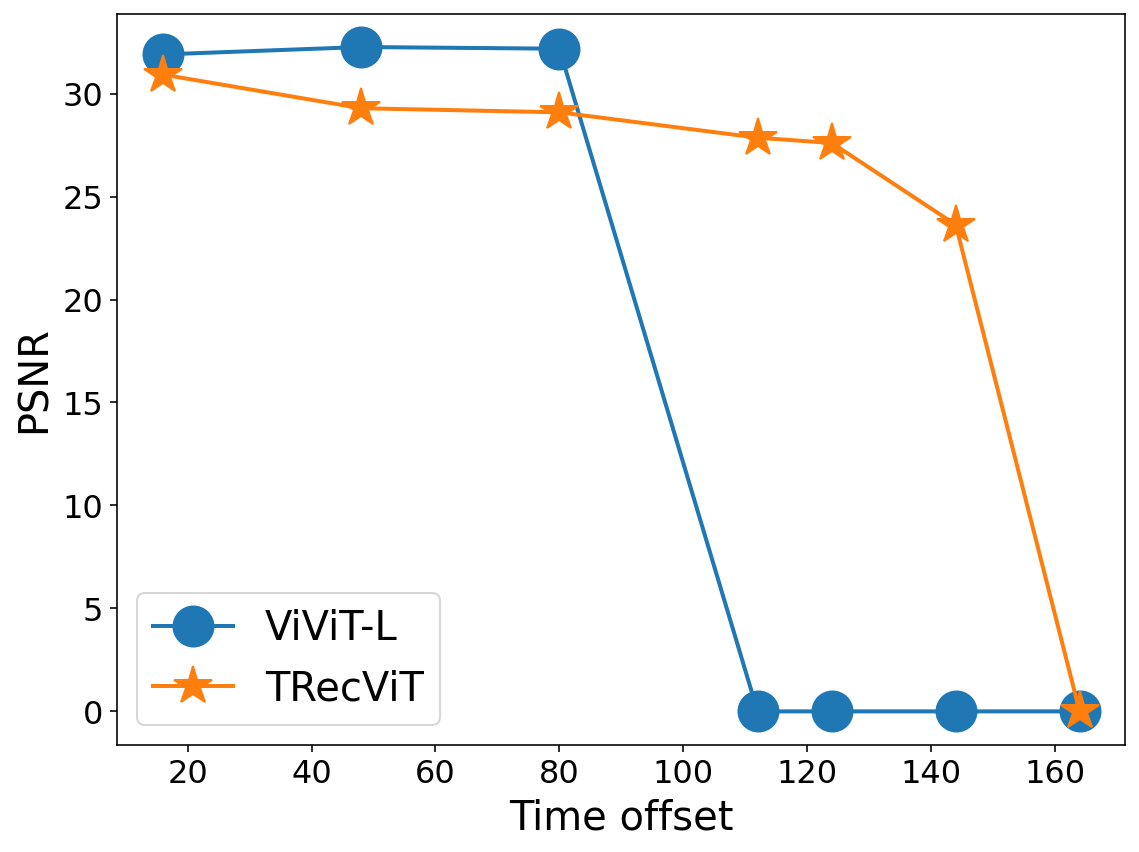
\includegraphics[width=\textwidth]{img/psnr.png}
    \caption{PSNR comparison}
\end{subfigure}%
\hfill
\begin{subfigure}{0.48\linewidth}
    \centering
    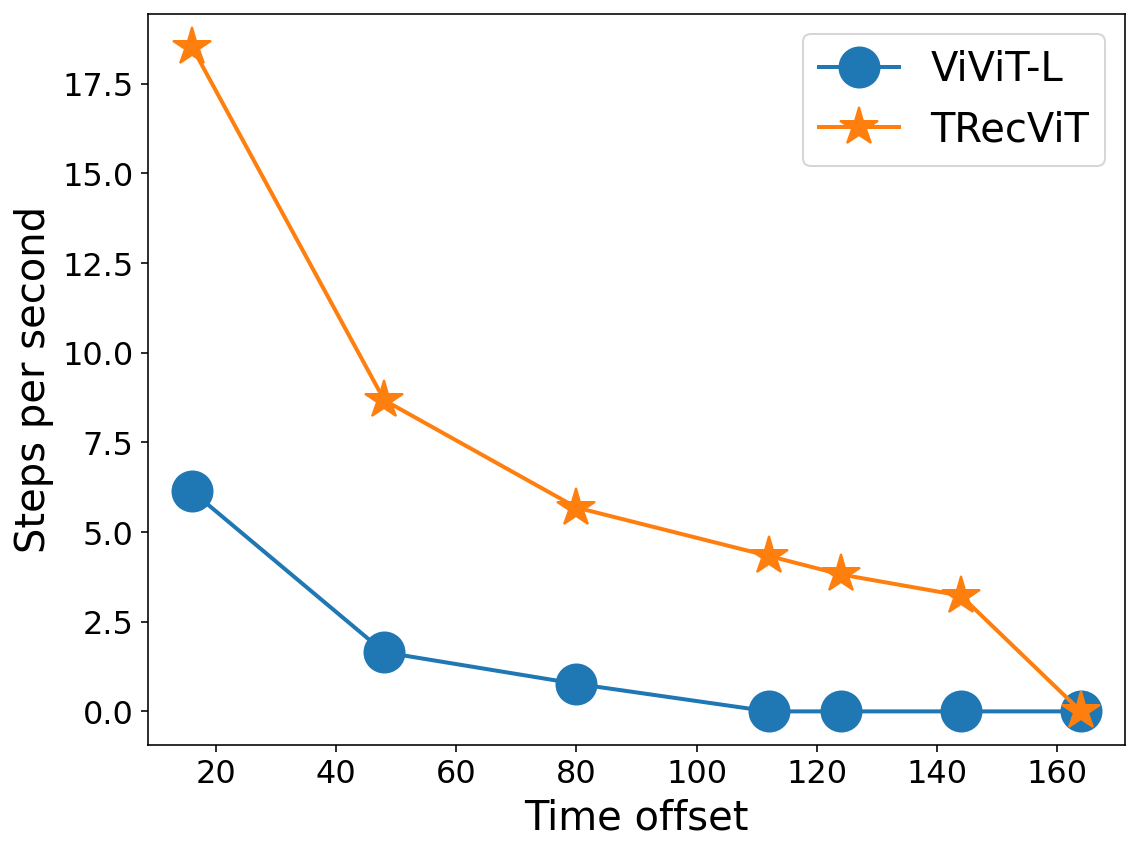
\includegraphics[width=\textwidth]{img/sps.png} 
    \caption{Steps-per-second comparison}
\end{subfigure}
\caption{Long video memorisation task. At time $T$, the model has to reconstruct the $(T-k)^\text{th}$ frame seen in the past. The plots show PSNR and throughput (steps-per-second) for increasing time offset $k$. For both models, the data points with $0$ value on the $y$-axis correspond to OOM.
}
\label{fig:psnr}
\end{figure}

\subsection{Long video memorisation task}
\label{sec:longtask}

Transformer models for language are known to be excellent at retrieving information from context, as they cache the keys and values for the entire history. On the other hand, LRUs / SSMs and RNNs in general struggle with such \emph{needle-in-the-haystack} style tasks as they need to perform the retrieval based on the compressed history kept in their recurrent state~\cite{jelassi2024repeat, de2024griffinmixinggatedlinear}. 
We are interested in studying this aspect in the video domain as well. We set up a simple reconstruction task where the model has to remember the frame seen at a given time-step in the past. For our analysis, we run multiple experiments where the model is tasked to reconstruct the $(T-k)^{\text{th}}$ frame from the past, with increasing value for $k\in\{16, 48, 80, 112, 144, 164\}$ frames. We employ Walking Tours dataset~\cite{venkataramanan2023imagenet}, which contains hour-long videos, and the scenery changes constantly, hence we are guaranteed that the video frames seen most recently will be very different compared to the frames seen earlier on. We scale the videos to $224\times224$ pixels. Again, we adopt ViViT-L as baseline, and we train both models using Imagenet pretrained weights. For ViViT-L, we keep all the outputs from all $T$ time steps and apply temporal pooling and a $1\times1$ convolution to get the expected shape for the reconstructed frame. For \ssm, we simply keep the output of the last layer at time step $T$ and reshape it to the expected shape. We show quantitative and qualitative results respectively in Figures~\ref{fig:psnr} and~\ref{fig:wt}. We can observe that there is a performance--efficiency trade-off at play for \ssm: its performance is slightly below ViViT's for shorter memory spans (16, 48, 80), but its efficiency (steps-per-second) is significantly higher. However, beyond 80 frames, ViViT-L goes out of memory, whilst \ssm\ continues to give decent results up to 144 frames, going out of memory towards 164 frames. Figure~\ref{fig:wt} shows qualitative results compared to the baseline for the case where the models have to remember the frame seen at $T-48$ in the past. We can observe that the quality of ViViT-L's reconstruction is good. For \ssm, whilst the overall structure (encoded in lower frequencies) is correct, it struggles to remember the high-frequency content of the image. This is to be expected due to the compression happening in the recurrent state of the model. However, given how different the last seen frame is from the target frame, we consider this to be a very promising result that warrants further investigation into the memorisation capabilities of our model, which we leave as future work.

\subsection{Generalisation to longer sequences}
\label{sec:gentask}

Using the same task as above, we analyse the generalisation capabilities to sequences longer than those used during training. Specifically, we train the models with sequences of length $T=64$ frames to reconstruct the $T-48$ frame, and evaluate them on longer sequences $T=96$ to reconstruct the same frame. The \ssm\ model can run on longer sequences without any modification. For the ViViT model, we need to adapt the positional encoding to accommodate longer sequences. We use interpolation to nearest neighbour to obtain the desired length; cubic interpolation led to worse results. The performance of \ssm\ degrades slightly, with PSNR going down from 29.3 (when evaluated on the same sequence length as in training $T=64$) to 26.4 when evaluated with $T=96$ frame sequences. ViViT's PSNR, however, drops significantly, from 32.3 when evaluated on the same sequence length, to 15.1 when evaluated on longer sequences. We include qualitative examples in Figure~\ref{fig:gentask} where we can observe that ViViT's output contains stronger artefacts compared to \ssm. 

\begin{figure}[h]
  \centering
  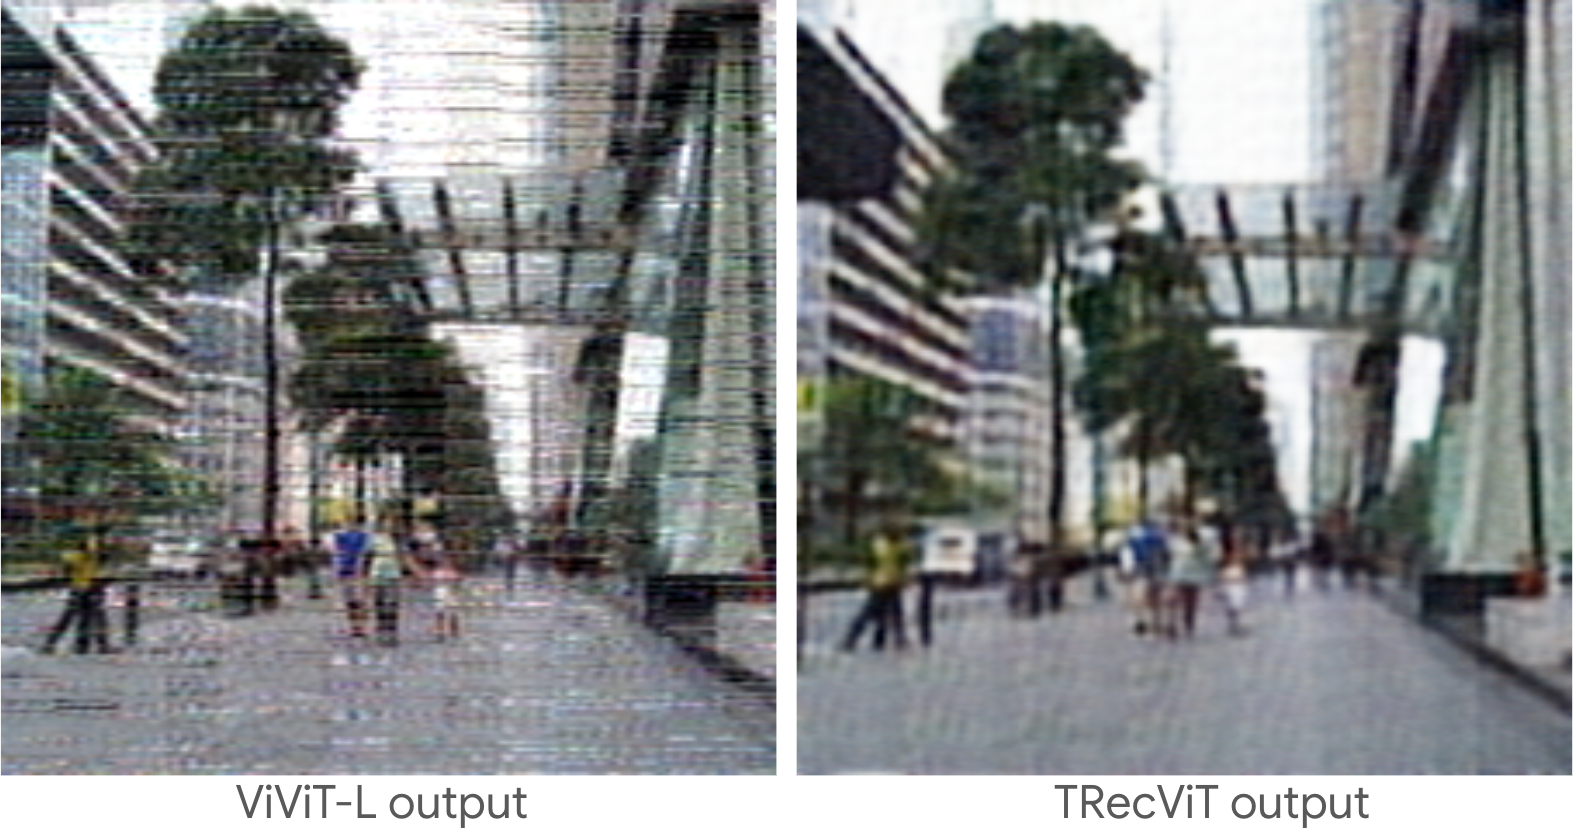
\includegraphics[width=\linewidth]{img/genlong.png}
  \caption{Generalisation to longer sequences. Both models are trained using Imagenet pre-trained weights, on video sequences of $T=64$ frames to reconstruct the $(T-48)^\text{th}$ frame; during evaluation, the models receive sequences of $T=96$ frames.}
  \label{fig:gentask}
\end{figure}

\section{Conclusion}
\label{sec:conclusion}
In this paper, we have investigated the common and unresolved issue that many established neural networks suffer from low floating-point operations per second (FLOPS). We have revisited a bottleneck operator, DWConv, and analyzed its main cause for a slowdown -- frequent memory access. To overcome the issue and achieve faster neural networks, we have proposed a simple yet fast and effective operator, PConv, that can be readily plugged into many existing networks. We have further introduced our general-purpose FasterNet, built upon our PConv, that achieves state-of-the-art speed and accuracy trade-off on various devices and vision tasks. We hope that our PConv and FasterNet would inspire more research on simple yet effective neural networks, going beyond academia to impact the industry and community directly.


{
    \small
    \bibliographystyle{ieeenat_fullname}
    \bibliography{main}
}


\end{document}
